% Created by tikzDevice version 0.12 on 2019-06-13 14:18:20
% !TEX encoding = UTF-8 Unicode
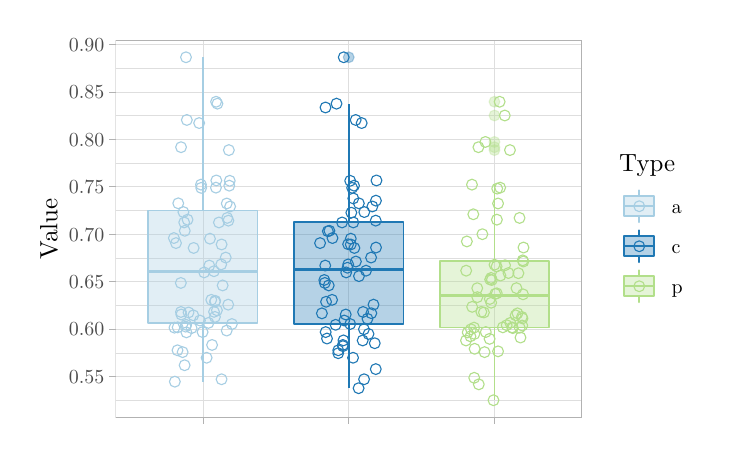
\begin{tikzpicture}[x=1pt,y=1pt]
\definecolor{fillColor}{RGB}{255,255,255}
\path[use as bounding box,fill=fillColor,fill opacity=0.00] (0,0) rectangle (245.72,151.77);
\begin{scope}
\path[clip] (  0.00,  0.00) rectangle (245.72,151.77);
\definecolor{drawColor}{RGB}{255,255,255}
\definecolor{fillColor}{RGB}{255,255,255}

\path[draw=drawColor,line width= 0.5pt,line join=round,line cap=round,fill=fillColor] (  0.00,  0.00) rectangle (245.72,151.77);
\end{scope}
\begin{scope}
\path[clip] ( 31.74, 10.94) rectangle (200.26,147.27);
\definecolor{fillColor}{RGB}{255,255,255}

\path[fill=fillColor] ( 31.74, 10.94) rectangle (200.26,147.27);
\definecolor{drawColor}{gray}{0.87}

\path[draw=drawColor,line width= 0.1pt,line join=round] ( 31.74, 17.12) --
	(200.26, 17.12);

\path[draw=drawColor,line width= 0.1pt,line join=round] ( 31.74, 34.27) --
	(200.26, 34.27);

\path[draw=drawColor,line width= 0.1pt,line join=round] ( 31.74, 51.42) --
	(200.26, 51.42);

\path[draw=drawColor,line width= 0.1pt,line join=round] ( 31.74, 68.56) --
	(200.26, 68.56);

\path[draw=drawColor,line width= 0.1pt,line join=round] ( 31.74, 85.71) --
	(200.26, 85.71);

\path[draw=drawColor,line width= 0.1pt,line join=round] ( 31.74,102.86) --
	(200.26,102.86);

\path[draw=drawColor,line width= 0.1pt,line join=round] ( 31.74,120.01) --
	(200.26,120.01);

\path[draw=drawColor,line width= 0.1pt,line join=round] ( 31.74,137.16) --
	(200.26,137.16);

\path[draw=drawColor,line width= 0.2pt,line join=round] ( 31.74, 25.69) --
	(200.26, 25.69);

\path[draw=drawColor,line width= 0.2pt,line join=round] ( 31.74, 42.84) --
	(200.26, 42.84);

\path[draw=drawColor,line width= 0.2pt,line join=round] ( 31.74, 59.99) --
	(200.26, 59.99);

\path[draw=drawColor,line width= 0.2pt,line join=round] ( 31.74, 77.14) --
	(200.26, 77.14);

\path[draw=drawColor,line width= 0.2pt,line join=round] ( 31.74, 94.29) --
	(200.26, 94.29);

\path[draw=drawColor,line width= 0.2pt,line join=round] ( 31.74,111.43) --
	(200.26,111.43);

\path[draw=drawColor,line width= 0.2pt,line join=round] ( 31.74,128.58) --
	(200.26,128.58);

\path[draw=drawColor,line width= 0.2pt,line join=round] ( 31.74,145.73) --
	(200.26,145.73);

\path[draw=drawColor,line width= 0.2pt,line join=round] ( 63.34, 10.94) --
	( 63.34,147.27);

\path[draw=drawColor,line width= 0.2pt,line join=round] (116.00, 10.94) --
	(116.00,147.27);

\path[draw=drawColor,line width= 0.2pt,line join=round] (168.67, 10.94) --
	(168.67,147.27);
\definecolor{drawColor}{RGB}{166,206,227}

\path[draw=drawColor,line width= 0.6pt,line join=round] ( 63.34, 85.65) -- ( 63.34,141.07);

\path[draw=drawColor,line width= 0.6pt,line join=round] ( 63.34, 44.99) -- ( 63.34, 23.85);
\definecolor{fillColor}{RGB}{166,206,227}

\path[draw=drawColor,line width= 0.6pt,line join=round,line cap=round,fill=fillColor,fill opacity=0.33] ( 43.59, 85.65) --
	( 43.59, 44.99) --
	( 83.09, 44.99) --
	( 83.09, 85.65) --
	( 43.59, 85.65) --
	cycle;

\path[draw=drawColor,line width= 1.1pt,line join=round] ( 43.59, 63.54) -- ( 83.09, 63.54);
\definecolor{drawColor}{RGB}{31,120,180}
\definecolor{fillColor}{RGB}{31,120,180}

\path[draw=drawColor,draw opacity=0.33,line width= 0.4pt,line join=round,line cap=round,fill=fillColor,fill opacity=0.33] (116.00,141.07) circle (  1.96);
\definecolor{drawColor}{RGB}{31,120,180}

\path[draw=drawColor,line width= 0.6pt,line join=round] (116.00, 81.55) -- (116.00,124.31);

\path[draw=drawColor,line width= 0.6pt,line join=round] (116.00, 44.61) -- (116.00, 21.49);

\path[draw=drawColor,line width= 0.6pt,line join=round,line cap=round,fill=fillColor,fill opacity=0.33] ( 96.25, 81.55) --
	( 96.25, 44.61) --
	(135.75, 44.61) --
	(135.75, 81.55) --
	( 96.25, 81.55) --
	cycle;

\path[draw=drawColor,line width= 1.1pt,line join=round] ( 96.25, 64.49) -- (135.75, 64.49);
\definecolor{drawColor}{RGB}{178,223,138}
\definecolor{fillColor}{RGB}{178,223,138}

\path[draw=drawColor,draw opacity=0.33,line width= 0.4pt,line join=round,line cap=round,fill=fillColor,fill opacity=0.33] (168.67,125.00) circle (  1.96);

\path[draw=drawColor,draw opacity=0.33,line width= 0.4pt,line join=round,line cap=round,fill=fillColor,fill opacity=0.33] (168.67,107.53) circle (  1.96);

\path[draw=drawColor,draw opacity=0.33,line width= 0.4pt,line join=round,line cap=round,fill=fillColor,fill opacity=0.33] (168.67,120.03) circle (  1.96);

\path[draw=drawColor,draw opacity=0.33,line width= 0.4pt,line join=round,line cap=round,fill=fillColor,fill opacity=0.33] (168.67,108.58) circle (  1.96);

\path[draw=drawColor,draw opacity=0.33,line width= 0.4pt,line join=round,line cap=round,fill=fillColor,fill opacity=0.33] (168.67,110.47) circle (  1.96);
\definecolor{drawColor}{RGB}{178,223,138}

\path[draw=drawColor,line width= 0.6pt,line join=round] (168.67, 67.37) -- (168.67, 95.05);

\path[draw=drawColor,line width= 0.6pt,line join=round] (168.67, 43.37) -- (168.67, 17.14);

\path[draw=drawColor,line width= 0.6pt,line join=round,line cap=round,fill=fillColor,fill opacity=0.33] (148.92, 67.37) --
	(148.92, 43.37) --
	(188.42, 43.37) --
	(188.42, 67.37) --
	(148.92, 67.37) --
	cycle;

\path[draw=drawColor,line width= 1.1pt,line join=round] (148.92, 54.91) -- (188.42, 54.91);
\definecolor{drawColor}{RGB}{166,206,227}

\path[draw=drawColor,line width= 0.4pt,line join=round,line cap=round] ( 59.24, 43.21) circle (  1.96);

\path[draw=drawColor,line width= 0.4pt,line join=round,line cap=round] ( 68.08,125.00) circle (  1.96);

\path[draw=drawColor,line width= 0.4pt,line join=round,line cap=round] ( 66.63, 37.12) circle (  1.96);

\path[draw=drawColor,line width= 0.4pt,line join=round,line cap=round] ( 72.70,107.53) circle (  1.96);

\path[draw=drawColor,line width= 0.4pt,line join=round,line cap=round] ( 66.35, 53.42) circle (  1.96);

\path[draw=drawColor,line width= 0.4pt,line join=round,line cap=round] ( 68.03, 93.96) circle (  1.96);

\path[draw=drawColor,line width= 0.4pt,line join=round,line cap=round] ( 53.59, 73.93) circle (  1.96);

\path[draw=drawColor,line width= 0.4pt,line join=round,line cap=round] ( 55.38, 49.04) circle (  1.96);

\path[draw=drawColor,line width= 0.4pt,line join=round,line cap=round] ( 67.66, 47.25) circle (  1.96);

\path[draw=drawColor,line width= 0.4pt,line join=round,line cap=round] ( 67.35, 49.08) circle (  1.96);
\definecolor{drawColor}{RGB}{31,120,180}

\path[draw=drawColor,line width= 0.4pt,line join=round,line cap=round] (112.22, 34.13) circle (  1.96);

\path[draw=drawColor,line width= 0.4pt,line join=round,line cap=round] (107.62,122.93) circle (  1.96);

\path[draw=drawColor,line width= 0.4pt,line join=round,line cap=round] (113.89, 37.12) circle (  1.96);

\path[draw=drawColor,line width= 0.4pt,line join=round,line cap=round] (115.80, 73.52) circle (  1.96);

\path[draw=drawColor,line width= 0.4pt,line join=round,line cap=round] (109.99, 53.42) circle (  1.96);

\path[draw=drawColor,line width= 0.4pt,line join=round,line cap=round] (117.66, 90.07) circle (  1.96);

\path[draw=drawColor,line width= 0.4pt,line join=round,line cap=round] (105.66, 73.93) circle (  1.96);

\path[draw=drawColor,line width= 0.4pt,line join=round,line cap=round] (121.20, 49.04) circle (  1.96);

\path[draw=drawColor,line width= 0.4pt,line join=round,line cap=round] (122.79, 46.58) circle (  1.96);

\path[draw=drawColor,line width= 0.4pt,line join=round,line cap=round] (108.16, 39.44) circle (  1.96);
\definecolor{drawColor}{RGB}{178,223,138}

\path[draw=drawColor,line width= 0.4pt,line join=round,line cap=round] (175.30, 43.21) circle (  1.96);

\path[draw=drawColor,line width= 0.4pt,line join=round,line cap=round] (170.54,125.00) circle (  1.96);

\path[draw=drawColor,line width= 0.4pt,line join=round,line cap=round] (165.10, 34.53) circle (  1.96);

\path[draw=drawColor,line width= 0.4pt,line join=round,line cap=round] (174.27,107.53) circle (  1.96);

\path[draw=drawColor,line width= 0.4pt,line join=round,line cap=round] (178.72, 44.14) circle (  1.96);

\path[draw=drawColor,line width= 0.4pt,line join=round,line cap=round] (170.73, 93.96) circle (  1.96);

\path[draw=drawColor,line width= 0.4pt,line join=round,line cap=round] (168.69, 66.11) circle (  1.96);

\path[draw=drawColor,line width= 0.4pt,line join=round,line cap=round] (173.09, 44.27) circle (  1.96);

\path[draw=drawColor,line width= 0.4pt,line join=round,line cap=round] (178.58, 47.25) circle (  1.96);

\path[draw=drawColor,line width= 0.4pt,line join=round,line cap=round] (163.93, 49.08) circle (  1.96);
\definecolor{drawColor}{RGB}{166,206,227}

\path[draw=drawColor,line width= 0.4pt,line join=round,line cap=round] ( 53.04, 43.37) circle (  1.96);

\path[draw=drawColor,line width= 0.4pt,line join=round,line cap=round] ( 68.56,124.31) circle (  1.96);

\path[draw=drawColor,line width= 0.4pt,line join=round,line cap=round] ( 55.42,108.58) circle (  1.96);

\path[draw=drawColor,line width= 0.4pt,line join=round,line cap=round] ( 67.66, 52.72) circle (  1.96);

\path[draw=drawColor,line width= 0.4pt,line join=round,line cap=round] ( 62.62, 95.05) circle (  1.96);

\path[draw=drawColor,line width= 0.4pt,line join=round,line cap=round] ( 70.07, 73.43) circle (  1.96);

\path[draw=drawColor,line width= 0.4pt,line join=round,line cap=round] ( 55.51, 48.12) circle (  1.96);

\path[draw=drawColor,line width= 0.4pt,line join=round,line cap=round] ( 58.13, 48.86) circle (  1.96);

\path[draw=drawColor,line width= 0.4pt,line join=round,line cap=round] ( 59.85, 47.83) circle (  1.96);
\definecolor{drawColor}{RGB}{31,120,180}

\path[draw=drawColor,line width= 0.4pt,line join=round,line cap=round] (114.10, 38.76) circle (  1.96);

\path[draw=drawColor,line width= 0.4pt,line join=round,line cap=round] (111.60,124.31) circle (  1.96);

\path[draw=drawColor,line width= 0.4pt,line join=round,line cap=round] (108.47, 78.21) circle (  1.96);

\path[draw=drawColor,line width= 0.4pt,line join=round,line cap=round] (107.82, 52.72) circle (  1.96);

\path[draw=drawColor,line width= 0.4pt,line join=round,line cap=round] (125.84, 89.26) circle (  1.96);

\path[draw=drawColor,line width= 0.4pt,line join=round,line cap=round] (116.75, 73.43) circle (  1.96);

\path[draw=drawColor,line width= 0.4pt,line join=round,line cap=round] (114.93, 48.12) circle (  1.96);

\path[draw=drawColor,line width= 0.4pt,line join=round,line cap=round] (124.18, 48.59) circle (  1.96);

\path[draw=drawColor,line width= 0.4pt,line join=round,line cap=round] (125.42, 37.74) circle (  1.96);
\definecolor{drawColor}{RGB}{178,223,138}

\path[draw=drawColor,line width= 0.4pt,line join=round,line cap=round] (161.29, 43.37) circle (  1.96);

\path[draw=drawColor,line width= 0.4pt,line join=round,line cap=round] (172.40,120.03) circle (  1.96);

\path[draw=drawColor,line width= 0.4pt,line join=round,line cap=round] (162.88,108.58) circle (  1.96);

\path[draw=drawColor,line width= 0.4pt,line join=round,line cap=round] (177.81, 43.37) circle (  1.96);

\path[draw=drawColor,line width= 0.4pt,line join=round,line cap=round] (160.55, 95.05) circle (  1.96);

\path[draw=drawColor,line width= 0.4pt,line join=round,line cap=round] (178.88, 67.69) circle (  1.96);

\path[draw=drawColor,line width= 0.4pt,line join=round,line cap=round] (166.91, 39.32) circle (  1.96);

\path[draw=drawColor,line width= 0.4pt,line join=round,line cap=round] (164.86, 48.86) circle (  1.96);

\path[draw=drawColor,line width= 0.4pt,line join=round,line cap=round] (176.32, 47.83) circle (  1.96);
\definecolor{drawColor}{RGB}{166,206,227}

\path[draw=drawColor,line width= 0.4pt,line join=round,line cap=round] ( 70.45, 58.63) circle (  1.96);

\path[draw=drawColor,line width= 0.4pt,line join=round,line cap=round] ( 72.85, 94.68) circle (  1.96);

\path[draw=drawColor,line width= 0.4pt,line join=round,line cap=round] ( 67.31, 63.76) circle (  1.96);

\path[draw=drawColor,line width= 0.4pt,line join=round,line cap=round] ( 54.41, 88.30) circle (  1.96);

\path[draw=drawColor,line width= 0.4pt,line join=round,line cap=round] ( 72.46, 51.68) circle (  1.96);

\path[draw=drawColor,line width= 0.4pt,line join=round,line cap=round] ( 52.83, 75.75) circle (  1.96);

\path[draw=drawColor,line width= 0.4pt,line join=round,line cap=round] ( 65.63, 65.81) circle (  1.96);

\path[draw=drawColor,line width= 0.4pt,line join=round,line cap=round] ( 62.23, 45.95) circle (  1.96);

\path[draw=drawColor,line width= 0.4pt,line join=round,line cap=round] ( 71.93, 88.24) circle (  1.96);

\path[draw=drawColor,line width= 0.4pt,line join=round,line cap=round] ( 69.11, 81.38) circle (  1.96);

\path[draw=drawColor,line width= 0.4pt,line join=round,line cap=round] ( 64.66, 32.50) circle (  1.96);
\definecolor{drawColor}{RGB}{31,120,180}

\path[draw=drawColor,line width= 0.4pt,line join=round,line cap=round] (108.78, 58.63) circle (  1.96);

\path[draw=drawColor,line width= 0.4pt,line join=round,line cap=round] (117.93, 94.68) circle (  1.96);

\path[draw=drawColor,line width= 0.4pt,line join=round,line cap=round] (125.87, 72.32) circle (  1.96);

\path[draw=drawColor,line width= 0.4pt,line join=round,line cap=round] (119.67, 88.30) circle (  1.96);

\path[draw=drawColor,line width= 0.4pt,line join=round,line cap=round] (124.97, 51.68) circle (  1.96);

\path[draw=drawColor,line width= 0.4pt,line join=round,line cap=round] (110.14, 75.75) circle (  1.96);

\path[draw=drawColor,line width= 0.4pt,line join=round,line cap=round] (107.53, 65.81) circle (  1.96);

\path[draw=drawColor,line width= 0.4pt,line join=round,line cap=round] (114.40, 45.95) circle (  1.96);

\path[draw=drawColor,line width= 0.4pt,line join=round,line cap=round] (116.96, 84.91) circle (  1.96);

\path[draw=drawColor,line width= 0.4pt,line join=round,line cap=round] (113.61, 81.38) circle (  1.96);

\path[draw=drawColor,line width= 0.4pt,line join=round,line cap=round] (117.57, 32.50) circle (  1.96);
\definecolor{drawColor}{RGB}{178,223,138}

\path[draw=drawColor,line width= 0.4pt,line join=round,line cap=round] (165.54, 41.79) circle (  1.96);

\path[draw=drawColor,line width= 0.4pt,line join=round,line cap=round] (167.48, 52.38) circle (  1.96);

\path[draw=drawColor,line width= 0.4pt,line join=round,line cap=round] (179.16, 72.32) circle (  1.96);

\path[draw=drawColor,line width= 0.4pt,line join=round,line cap=round] (158.70, 74.53) circle (  1.96);

\path[draw=drawColor,line width= 0.4pt,line join=round,line cap=round] (169.97, 34.81) circle (  1.96);

\path[draw=drawColor,line width= 0.4pt,line join=round,line cap=round] (172.50, 65.92) circle (  1.96);

\path[draw=drawColor,line width= 0.4pt,line join=round,line cap=round] (167.12, 60.77) circle (  1.96);

\path[draw=drawColor,line width= 0.4pt,line join=round,line cap=round] (178.08, 39.80) circle (  1.96);

\path[draw=drawColor,line width= 0.4pt,line join=round,line cap=round] (169.97, 88.24) circle (  1.96);

\path[draw=drawColor,line width= 0.4pt,line join=round,line cap=round] (168.95, 55.58) circle (  1.96);

\path[draw=drawColor,line width= 0.4pt,line join=round,line cap=round] (163.01, 22.89) circle (  1.96);
\definecolor{drawColor}{RGB}{166,206,227}

\path[draw=drawColor,line width= 0.4pt,line join=round,line cap=round] ( 72.52, 82.04) circle (  1.96);

\path[draw=drawColor,line width= 0.4pt,line join=round,line cap=round] ( 57.51,118.42) circle (  1.96);

\path[draw=drawColor,line width= 0.4pt,line join=round,line cap=round] ( 68.17, 96.56) circle (  1.96);

\path[draw=drawColor,line width= 0.4pt,line join=round,line cap=round] ( 61.97,117.30) circle (  1.96);

\path[draw=drawColor,line width= 0.4pt,line join=round,line cap=round] ( 73.15, 87.16) circle (  1.96);

\path[draw=drawColor,line width= 0.4pt,line join=round,line cap=round] ( 59.97, 72.17) circle (  1.96);

\path[draw=drawColor,line width= 0.4pt,line join=round,line cap=round] ( 63.20, 41.77) circle (  1.96);

\path[draw=drawColor,line width= 0.4pt,line join=round,line cap=round] ( 63.78, 63.33) circle (  1.96);

\path[draw=drawColor,line width= 0.4pt,line join=round,line cap=round] ( 72.12, 83.02) circle (  1.96);

\path[draw=drawColor,line width= 0.4pt,line join=round,line cap=round] ( 73.02, 96.44) circle (  1.96);

\path[draw=drawColor,line width= 0.4pt,line join=round,line cap=round] ( 56.56, 81.39) circle (  1.96);
\definecolor{drawColor}{RGB}{31,120,180}

\path[draw=drawColor,line width= 0.4pt,line join=round,line cap=round] (125.77, 82.04) circle (  1.96);

\path[draw=drawColor,line width= 0.4pt,line join=round,line cap=round] (118.52,118.42) circle (  1.96);

\path[draw=drawColor,line width= 0.4pt,line join=round,line cap=round] (126.04, 96.56) circle (  1.96);

\path[draw=drawColor,line width= 0.4pt,line join=round,line cap=round] (120.69,117.30) circle (  1.96);

\path[draw=drawColor,line width= 0.4pt,line join=round,line cap=round] (124.56, 87.16) circle (  1.96);

\path[draw=drawColor,line width= 0.4pt,line join=round,line cap=round] (118.06, 72.17) circle (  1.96);

\path[draw=drawColor,line width= 0.4pt,line join=round,line cap=round] (107.68, 41.77) circle (  1.96);

\path[draw=drawColor,line width= 0.4pt,line join=round,line cap=round] (115.10, 63.33) circle (  1.96);

\path[draw=drawColor,line width= 0.4pt,line join=round,line cap=round] (115.56, 65.02) circle (  1.96);

\path[draw=drawColor,line width= 0.4pt,line join=round,line cap=round] (116.54, 96.44) circle (  1.96);

\path[draw=drawColor,line width= 0.4pt,line join=round,line cap=round] (117.67, 81.39) circle (  1.96);
\definecolor{drawColor}{RGB}{178,223,138}

\path[draw=drawColor,line width= 0.4pt,line join=round,line cap=round] (160.62, 50.89) circle (  1.96);

\path[draw=drawColor,line width= 0.4pt,line join=round,line cap=round] (161.03, 84.34) circle (  1.96);

\path[draw=drawColor,line width= 0.4pt,line join=round,line cap=round] (167.45, 61.34) circle (  1.96);

\path[draw=drawColor,line width= 0.4pt,line join=round,line cap=round] (165.40,110.47) circle (  1.96);

\path[draw=drawColor,line width= 0.4pt,line join=round,line cap=round] (176.63, 57.65) circle (  1.96);

\path[draw=drawColor,line width= 0.4pt,line join=round,line cap=round] (170.84, 62.20) circle (  1.96);

\path[draw=drawColor,line width= 0.4pt,line join=round,line cap=round] (159.98, 40.24) circle (  1.96);

\path[draw=drawColor,line width= 0.4pt,line join=round,line cap=round] (162.48, 54.39) circle (  1.96);

\path[draw=drawColor,line width= 0.4pt,line join=round,line cap=round] (177.74, 83.02) circle (  1.96);

\path[draw=drawColor,line width= 0.4pt,line join=round,line cap=round] (173.73, 63.11) circle (  1.96);

\path[draw=drawColor,line width= 0.4pt,line join=round,line cap=round] (164.31, 77.14) circle (  1.96);
\definecolor{drawColor}{RGB}{166,206,227}

\path[draw=drawColor,line width= 0.4pt,line join=round,line cap=round] ( 68.39, 49.65) circle (  1.96);

\path[draw=drawColor,line width= 0.4pt,line join=round,line cap=round] ( 53.18, 23.85) circle (  1.96);

\path[draw=drawColor,line width= 0.4pt,line join=round,line cap=round] ( 56.77, 78.37) circle (  1.96);

\path[draw=drawColor,line width= 0.4pt,line join=round,line cap=round] ( 56.28, 85.14) circle (  1.96);

\path[draw=drawColor,line width= 0.4pt,line join=round,line cap=round] ( 57.77, 82.39) circle (  1.96);

\path[draw=drawColor,line width= 0.4pt,line join=round,line cap=round] ( 56.71, 29.79) circle (  1.96);

\path[draw=drawColor,line width= 0.4pt,line join=round,line cap=round] ( 55.34, 59.53) circle (  1.96);

\path[draw=drawColor,line width= 0.4pt,line join=round,line cap=round] ( 55.99, 34.53) circle (  1.96);

\path[draw=drawColor,line width= 0.4pt,line join=round,line cap=round] ( 70.06, 24.72) circle (  1.96);

\path[draw=drawColor,line width= 0.4pt,line join=round,line cap=round] ( 57.08, 43.75) circle (  1.96);

\path[draw=drawColor,line width= 0.4pt,line join=round,line cap=round] ( 57.26, 44.40) circle (  1.96);
\definecolor{drawColor}{RGB}{31,120,180}

\path[draw=drawColor,line width= 0.4pt,line join=round,line cap=round] (122.27, 63.96) circle (  1.96);

\path[draw=drawColor,line width= 0.4pt,line join=round,line cap=round] (123.16, 41.10) circle (  1.96);

\path[draw=drawColor,line width= 0.4pt,line join=round,line cap=round] (109.03, 78.37) circle (  1.96);

\path[draw=drawColor,line width= 0.4pt,line join=round,line cap=round] (121.64, 85.14) circle (  1.96);

\path[draw=drawColor,line width= 0.4pt,line join=round,line cap=round] (119.71, 61.99) circle (  1.96);

\path[draw=drawColor,line width= 0.4pt,line join=round,line cap=round] (106.32, 48.54) circle (  1.96);

\path[draw=drawColor,line width= 0.4pt,line join=round,line cap=round] (107.38, 59.53) circle (  1.96);

\path[draw=drawColor,line width= 0.4pt,line join=round,line cap=round] (121.05, 38.74) circle (  1.96);

\path[draw=drawColor,line width= 0.4pt,line join=round,line cap=round] (121.56, 24.72) circle (  1.96);

\path[draw=drawColor,line width= 0.4pt,line join=round,line cap=round] (118.60, 67.27) circle (  1.96);

\path[draw=drawColor,line width= 0.4pt,line join=round,line cap=round] (111.27, 44.40) circle (  1.96);
\definecolor{drawColor}{RGB}{178,223,138}

\path[draw=drawColor,line width= 0.4pt,line join=round,line cap=round] (158.45, 63.96) circle (  1.96);

\path[draw=drawColor,line width= 0.4pt,line join=round,line cap=round] (161.44, 41.10) circle (  1.96);

\path[draw=drawColor,line width= 0.4pt,line join=round,line cap=round] (169.51, 55.78) circle (  1.96);

\path[draw=drawColor,line width= 0.4pt,line join=round,line cap=round] (178.99, 55.42) circle (  1.96);

\path[draw=drawColor,line width= 0.4pt,line join=round,line cap=round] (169.55, 82.39) circle (  1.96);

\path[draw=drawColor,line width= 0.4pt,line join=round,line cap=round] (176.99, 48.54) circle (  1.96);

\path[draw=drawColor,line width= 0.4pt,line join=round,line cap=round] (162.45, 57.63) circle (  1.96);

\path[draw=drawColor,line width= 0.4pt,line join=round,line cap=round] (158.38, 38.74) circle (  1.96);

\path[draw=drawColor,line width= 0.4pt,line join=round,line cap=round] (168.32, 17.14) circle (  1.96);

\path[draw=drawColor,line width= 0.4pt,line join=round,line cap=round] (179.12, 67.27) circle (  1.96);

\path[draw=drawColor,line width= 0.4pt,line join=round,line cap=round] (161.50, 35.73) circle (  1.96);
\definecolor{drawColor}{RGB}{166,206,227}

\path[draw=drawColor,line width= 0.4pt,line join=round,line cap=round] ( 71.56, 68.70) circle (  1.96);

\path[draw=drawColor,line width= 0.4pt,line join=round,line cap=round] ( 62.70, 93.89) circle (  1.96);

\path[draw=drawColor,line width= 0.4pt,line join=round,line cap=round] ( 71.92, 42.32) circle (  1.96);

\path[draw=drawColor,line width= 0.4pt,line join=round,line cap=round] ( 69.94, 66.23) circle (  1.96);

\path[draw=drawColor,line width= 0.4pt,line join=round,line cap=round] ( 57.21,141.07) circle (  1.96);

\path[draw=drawColor,line width= 0.4pt,line join=round,line cap=round] ( 65.87, 75.52) circle (  1.96);

\path[draw=drawColor,line width= 0.4pt,line join=round,line cap=round] ( 54.14, 35.19) circle (  1.96);

\path[draw=drawColor,line width= 0.4pt,line join=round,line cap=round] ( 67.76, 53.07) circle (  1.96);

\path[draw=drawColor,line width= 0.4pt,line join=round,line cap=round] ( 65.33, 45.09) circle (  1.96);

\path[draw=drawColor,line width= 0.4pt,line join=round,line cap=round] ( 54.20, 43.49) circle (  1.96);

\path[draw=drawColor,line width= 0.4pt,line join=round,line cap=round] ( 73.80, 44.68) circle (  1.96);
\definecolor{drawColor}{RGB}{31,120,180}

\path[draw=drawColor,line width= 0.4pt,line join=round,line cap=round] (124.09, 68.70) circle (  1.96);

\path[draw=drawColor,line width= 0.4pt,line join=round,line cap=round] (117.26, 93.89) circle (  1.96);

\path[draw=drawColor,line width= 0.4pt,line join=round,line cap=round] (121.51, 42.79) circle (  1.96);

\path[draw=drawColor,line width= 0.4pt,line join=round,line cap=round] (115.82, 66.23) circle (  1.96);

\path[draw=drawColor,line width= 0.4pt,line join=round,line cap=round] (114.21,141.07) circle (  1.96);

\path[draw=drawColor,line width= 0.4pt,line join=round,line cap=round] (116.76, 75.52) circle (  1.96);

\path[draw=drawColor,line width= 0.4pt,line join=round,line cap=round] (112.23, 35.19) circle (  1.96);

\path[draw=drawColor,line width= 0.4pt,line join=round,line cap=round] (107.19, 60.59) circle (  1.96);

\path[draw=drawColor,line width= 0.4pt,line join=round,line cap=round] (113.93, 36.68) circle (  1.96);

\path[draw=drawColor,line width= 0.4pt,line join=round,line cap=round] (119.58, 21.49) circle (  1.96);

\path[draw=drawColor,line width= 0.4pt,line join=round,line cap=round] (116.54, 44.68) circle (  1.96);
\definecolor{drawColor}{RGB}{178,223,138}

\path[draw=drawColor,line width= 0.4pt,line join=round,line cap=round] (178.80, 46.71) circle (  1.96);

\path[draw=drawColor,line width= 0.4pt,line join=round,line cap=round] (177.33, 63.04) circle (  1.96);

\path[draw=drawColor,line width= 0.4pt,line join=round,line cap=round] (160.18, 42.79) circle (  1.96);

\path[draw=drawColor,line width= 0.4pt,line join=round,line cap=round] (166.99, 53.73) circle (  1.96);

\path[draw=drawColor,line width= 0.4pt,line join=round,line cap=round] (169.66, 93.62) circle (  1.96);

\path[draw=drawColor,line width= 0.4pt,line join=round,line cap=round] (169.44, 65.49) circle (  1.96);

\path[draw=drawColor,line width= 0.4pt,line join=round,line cap=round] (161.36, 25.25) circle (  1.96);

\path[draw=drawColor,line width= 0.4pt,line join=round,line cap=round] (167.71, 60.59) circle (  1.96);

\path[draw=drawColor,line width= 0.4pt,line join=round,line cap=round] (174.40, 45.09) circle (  1.96);

\path[draw=drawColor,line width= 0.4pt,line join=round,line cap=round] (171.70, 43.49) circle (  1.96);

\path[draw=drawColor,line width= 0.4pt,line join=round,line cap=round] (175.06, 43.46) circle (  1.96);
\definecolor{drawColor}{RGB}{166,206,227}

\path[draw=drawColor,line width= 0.4pt,line join=round,line cap=round] ( 57.36, 41.67) circle (  1.96);
\definecolor{drawColor}{RGB}{31,120,180}

\path[draw=drawColor,line width= 0.4pt,line join=round,line cap=round] (125.79, 28.39) circle (  1.96);
\definecolor{drawColor}{RGB}{178,223,138}

\path[draw=drawColor,line width= 0.4pt,line join=round,line cap=round] (159.00, 41.67) circle (  1.96);
\definecolor{drawColor}{gray}{0.70}

\path[draw=drawColor,line width= 0.5pt,line join=round,line cap=round] ( 31.74, 10.94) rectangle (200.26,147.27);
\end{scope}
\begin{scope}
\path[clip] (  0.00,  0.00) rectangle (245.72,151.77);
\definecolor{drawColor}{gray}{0.30}

\node[text=drawColor,anchor=base east,inner sep=0pt, outer sep=0pt, scale=  0.72] at ( 27.69, 23.21) {0.55};

\node[text=drawColor,anchor=base east,inner sep=0pt, outer sep=0pt, scale=  0.72] at ( 27.69, 40.36) {0.60};

\node[text=drawColor,anchor=base east,inner sep=0pt, outer sep=0pt, scale=  0.72] at ( 27.69, 57.51) {0.65};

\node[text=drawColor,anchor=base east,inner sep=0pt, outer sep=0pt, scale=  0.72] at ( 27.69, 74.66) {0.70};

\node[text=drawColor,anchor=base east,inner sep=0pt, outer sep=0pt, scale=  0.72] at ( 27.69, 91.81) {0.75};

\node[text=drawColor,anchor=base east,inner sep=0pt, outer sep=0pt, scale=  0.72] at ( 27.69,108.96) {0.80};

\node[text=drawColor,anchor=base east,inner sep=0pt, outer sep=0pt, scale=  0.72] at ( 27.69,126.10) {0.85};

\node[text=drawColor,anchor=base east,inner sep=0pt, outer sep=0pt, scale=  0.72] at ( 27.69,143.25) {0.90};
\end{scope}
\begin{scope}
\path[clip] (  0.00,  0.00) rectangle (245.72,151.77);
\definecolor{drawColor}{gray}{0.70}

\path[draw=drawColor,line width= 0.2pt,line join=round] ( 29.49, 25.69) --
	( 31.74, 25.69);

\path[draw=drawColor,line width= 0.2pt,line join=round] ( 29.49, 42.84) --
	( 31.74, 42.84);

\path[draw=drawColor,line width= 0.2pt,line join=round] ( 29.49, 59.99) --
	( 31.74, 59.99);

\path[draw=drawColor,line width= 0.2pt,line join=round] ( 29.49, 77.14) --
	( 31.74, 77.14);

\path[draw=drawColor,line width= 0.2pt,line join=round] ( 29.49, 94.29) --
	( 31.74, 94.29);

\path[draw=drawColor,line width= 0.2pt,line join=round] ( 29.49,111.43) --
	( 31.74,111.43);

\path[draw=drawColor,line width= 0.2pt,line join=round] ( 29.49,128.58) --
	( 31.74,128.58);

\path[draw=drawColor,line width= 0.2pt,line join=round] ( 29.49,145.73) --
	( 31.74,145.73);
\end{scope}
\begin{scope}
\path[clip] (  0.00,  0.00) rectangle (245.72,151.77);
\definecolor{drawColor}{gray}{0.70}

\path[draw=drawColor,line width= 0.2pt,line join=round] ( 63.34,  8.69) --
	( 63.34, 10.94);

\path[draw=drawColor,line width= 0.2pt,line join=round] (116.00,  8.69) --
	(116.00, 10.94);

\path[draw=drawColor,line width= 0.2pt,line join=round] (168.67,  8.69) --
	(168.67, 10.94);
\end{scope}
\begin{scope}
\path[clip] (  0.00,  0.00) rectangle (245.72,151.77);
\definecolor{drawColor}{RGB}{0,0,0}

\node[text=drawColor,rotate= 90.00,anchor=base,inner sep=0pt, outer sep=0pt, scale=  0.90] at ( 10.70, 79.11) {Value};
\end{scope}
\begin{scope}
\path[clip] (  0.00,  0.00) rectangle (245.72,151.77);
\definecolor{fillColor}{RGB}{255,255,255}

\path[fill=fillColor] (209.26, 46.60) rectangle (241.22,111.61);
\end{scope}
\begin{scope}
\path[clip] (  0.00,  0.00) rectangle (245.72,151.77);
\definecolor{drawColor}{RGB}{0,0,0}

\node[text=drawColor,anchor=base west,inner sep=0pt, outer sep=0pt, scale=  0.90] at (213.76, 99.94) {Type};
\end{scope}
\begin{scope}
\path[clip] (  0.00,  0.00) rectangle (245.72,151.77);
\definecolor{fillColor}{RGB}{255,255,255}

\path[fill=fillColor] (213.76, 80.01) rectangle (228.22, 94.47);
\end{scope}
\begin{scope}
\path[clip] (  0.00,  0.00) rectangle (245.72,151.77);
\definecolor{drawColor}{RGB}{166,206,227}

\path[draw=drawColor,line width= 0.6pt,line join=round,line cap=round] (220.99, 81.46) --
	(220.99, 83.62);

\path[draw=drawColor,line width= 0.6pt,line join=round,line cap=round] (220.99, 90.85) --
	(220.99, 93.02);
\definecolor{fillColor}{RGB}{166,206,227}

\path[draw=drawColor,line width= 0.6pt,line join=round,line cap=round,fill=fillColor,fill opacity=0.33] (215.57, 83.62) rectangle (226.41, 90.85);

\path[draw=drawColor,line width= 0.6pt,line join=round,line cap=round] (215.57, 87.24) --
	(226.41, 87.24);
\end{scope}
\begin{scope}
\path[clip] (  0.00,  0.00) rectangle (245.72,151.77);
\definecolor{drawColor}{RGB}{166,206,227}

\path[draw=drawColor,line width= 0.4pt,line join=round,line cap=round] (220.99, 87.24) circle (  1.96);
\end{scope}
\begin{scope}
\path[clip] (  0.00,  0.00) rectangle (245.72,151.77);
\definecolor{fillColor}{RGB}{255,255,255}

\path[fill=fillColor] (213.76, 65.56) rectangle (228.22, 80.01);
\end{scope}
\begin{scope}
\path[clip] (  0.00,  0.00) rectangle (245.72,151.77);
\definecolor{drawColor}{RGB}{31,120,180}

\path[draw=drawColor,line width= 0.6pt,line join=round,line cap=round] (220.99, 67.00) --
	(220.99, 69.17);

\path[draw=drawColor,line width= 0.6pt,line join=round,line cap=round] (220.99, 76.40) --
	(220.99, 78.57);
\definecolor{fillColor}{RGB}{31,120,180}

\path[draw=drawColor,line width= 0.6pt,line join=round,line cap=round,fill=fillColor,fill opacity=0.33] (215.57, 69.17) rectangle (226.41, 76.40);

\path[draw=drawColor,line width= 0.6pt,line join=round,line cap=round] (215.57, 72.78) --
	(226.41, 72.78);
\end{scope}
\begin{scope}
\path[clip] (  0.00,  0.00) rectangle (245.72,151.77);
\definecolor{drawColor}{RGB}{31,120,180}

\path[draw=drawColor,line width= 0.4pt,line join=round,line cap=round] (220.99, 72.78) circle (  1.96);
\end{scope}
\begin{scope}
\path[clip] (  0.00,  0.00) rectangle (245.72,151.77);
\definecolor{fillColor}{RGB}{255,255,255}

\path[fill=fillColor] (213.76, 51.10) rectangle (228.22, 65.56);
\end{scope}
\begin{scope}
\path[clip] (  0.00,  0.00) rectangle (245.72,151.77);
\definecolor{drawColor}{RGB}{178,223,138}

\path[draw=drawColor,line width= 0.6pt,line join=round,line cap=round] (220.99, 52.55) --
	(220.99, 54.72);

\path[draw=drawColor,line width= 0.6pt,line join=round,line cap=round] (220.99, 61.94) --
	(220.99, 64.11);
\definecolor{fillColor}{RGB}{178,223,138}

\path[draw=drawColor,line width= 0.6pt,line join=round,line cap=round,fill=fillColor,fill opacity=0.33] (215.57, 54.72) rectangle (226.41, 61.94);

\path[draw=drawColor,line width= 0.6pt,line join=round,line cap=round] (215.57, 58.33) --
	(226.41, 58.33);
\end{scope}
\begin{scope}
\path[clip] (  0.00,  0.00) rectangle (245.72,151.77);
\definecolor{drawColor}{RGB}{178,223,138}

\path[draw=drawColor,line width= 0.4pt,line join=round,line cap=round] (220.99, 58.33) circle (  1.96);
\end{scope}
\begin{scope}
\path[clip] (  0.00,  0.00) rectangle (245.72,151.77);
\definecolor{drawColor}{RGB}{0,0,0}

\node[text=drawColor,anchor=base west,inner sep=0pt, outer sep=0pt, scale=  0.72] at (232.72, 84.76) {a};
\end{scope}
\begin{scope}
\path[clip] (  0.00,  0.00) rectangle (245.72,151.77);
\definecolor{drawColor}{RGB}{0,0,0}

\node[text=drawColor,anchor=base west,inner sep=0pt, outer sep=0pt, scale=  0.72] at (232.72, 70.30) {c};
\end{scope}
\begin{scope}
\path[clip] (  0.00,  0.00) rectangle (245.72,151.77);
\definecolor{drawColor}{RGB}{0,0,0}

\node[text=drawColor,anchor=base west,inner sep=0pt, outer sep=0pt, scale=  0.72] at (232.72, 55.85) {p};
\end{scope}
\end{tikzpicture}
